\documentclass[a4paper,11pt]{exam}
%\printanswers % pour imprimer les réponses (corrigé)
\noprintanswers % Pour ne pas imprimer les réponses (énoncé)
\addpoints % Pour compter les points
% \noaddpoints % pour ne pas compter les points
%\qformat{\textbf{\thequestion ) } }
%\qformat{\textbf{\thequestion )}} % Pour définir le style des questions (facultatif)
\usepackage{color} % définit une nouvelle couleur
\shadedsolutions % définit le style des réponses
% \framedsolutions % définit le style des réponses
\definecolor{SolutionColor}{rgb}{0.8,0.9,1} % bleu ciel
\renewcommand{\solutiontitle}{\noindent\textbf{Solution:}\par\noindent} % Définit le titre des solutions




\makeatletter

\def\maketitle{{\centering%
	\par{\huge\textbf{\@title}}%
	\par{\@date}%
	\par}}


\renewcommand{\thesubsection}{\Alph{subsection}.}   

\makeatother

\lhead{NOM Pr\'enom :}
\rhead{\textbf{Les r\'eponses doivent \^etre justifi\'ees et r\'edig\'ees}}
\cfoot{\thepage / \pageref{LastPage}}


%\usepackage{../../pas-math}
%\usepackage{../../moncours}


%\usepackage{pas-cours}
%-------------------------------------------------------------------------------
%          -Packages nécessaires pour écrire en Français et en UTF8-
%-------------------------------------------------------------------------------
\usepackage[utf8]{inputenc}
\usepackage[frenchb]{babel}
%\usepackage{numprint}
\usepackage[T1]{fontenc}
%\usepackage{lmodern}
\usepackage{textcomp}
\usepackage[french, boxed]{algorithm2e}
\usepackage{hyperref}


%-------------------------------------------------------------------------------

%-------------------------------------------------------------------------------
%                          -Outils de mise en forme-
%-------------------------------------------------------------------------------
\usepackage{hyperref}
\hypersetup{pdfstartview=XYZ}
%\usepackage{enumerate}
\usepackage{graphicx}
\usepackage{multicol}
\usepackage{tabularx}
\usepackage{multirow}
\usepackage{color}
\usepackage{eurosym}


\usepackage{anysize} %%pour pouvoir mettre les marges qu'on veut
%\marginsize{2.5cm}{2.5cm}{2.5cm}{2.5cm}

\usepackage{indentfirst} %%pour que les premier paragraphes soient aussi indentés
\usepackage{verbatim}
\usepackage{enumitem}
\usepackage{booktabs}
\usepackage[usenames,dvipsnames,svgnames,table]{xcolor}

\usepackage{variations}

%-------------------------------------------------------------------------------


%-------------------------------------------------------------------------------
%                  -Nécessaires pour écrire des mathématiques-
%-------------------------------------------------------------------------------
\usepackage{amsfonts}
\usepackage{amssymb}
\usepackage{amsmath}
\usepackage{amsthm}
\usepackage{tikz}
\usepackage{xlop}
\usepackage[output-decimal-marker={,}]{siunitx}
%-------------------------------------------------------------------------------

%-------------------------------------------------------------------------------
%                  -Nécessaires pour écrire des formules chimiquess-
%-------------------------------------------------------------------------------

\usepackage[version=4]{mhchem}

%-------------------------------------------------------------------------------
% Pour pouvoir exploiter les fichiers directement dans beamer
\newcommand{\pause}{\ }
%-------------------------------------------------------------------------------
%                    - Mise en forme avancée
%-------------------------------------------------------------------------------

\usepackage{ifthen}
\usepackage{ifmtarg}


\newcommand{\ifTrue}[2]{\ifthenelse{\equal{#1}{true}}{#2}{$\qquad \qquad$}}

%\newcommand{\kword}[1]{\textcolor{red}{\underline{#1}}}
%-------------------------------------------------------------------------------

%-------------------------------------------------------------------------------
%                     -Mise en forme d'exercices-
%-------------------------------------------------------------------------------
%\newtheoremstyle{exostyle}
%{\topsep}% espace avant
%{\topsep}% espace apres
%{}% Police utilisee par le style de thm
%{}% Indentation (vide = aucune, \parindent = indentation paragraphe)
%{\bfseries}% Police du titre de thm
%{.}% Signe de ponctuation apres le titre du thm
%{ }% Espace apres le titre du thm (\newline = linebreak)
%{\thmname{#1}\thmnumber{ #2}\thmnote{. \normalfont{\textit{#3}}}}% composants du titre du thm : \thmname = nom du thm, \thmnumber = numéro du thm, \thmnote = sous-titre du thm

%\theoremstyle{exostyle}
%\newtheorem{exercice}{Exercice}
%
%\newenvironment{questions}{
%\begin{enumerate}[\hspace{12pt}\bfseries\itshape a.]}{\end{enumerate}
%} %mettre un 1 à la place du a si on veut des numéros au lieu de lettres pour les questions 
%-------------------------------------------------------------------------------

%-------------------------------------------------------------------------------
%                    - Mise en forme de tableaux -
%-------------------------------------------------------------------------------

\renewcommand{\arraystretch}{1.7}

\setlength{\tabcolsep}{1.2cm}

%-------------------------------------------------------------------------------



%-------------------------------------------------------------------------------
%                    - Racourcis d'écriture -
%-------------------------------------------------------------------------------
%Droites
\newcommand{\dte}[1]{$(#1)$}
\newcommand{\fig}[1]{figure $#1$}
\newcommand{\sym}{symétrique}
\newcommand{\syms}{symétriques}
\newcommand{\asym}{axe de symétrie}
\newcommand{\asyms}{axes de symétrie}
\newcommand{\seg}[1]{$[#1]$}
\newcommand{\monAngle}[1]{$\widehat{#1}$}
\newcommand{\bissec}{bissectrice}
\newcommand{\mediat}{médiatrice}
\newcommand{\ddte}[1]{$[#1)$}


% Angles orientés (couples de vecteurs)
\newcommand{\aopp}[2]{(\vec{#1}, \vec{#2})} %Les deuc vecteurs sont positifs
\newcommand{\aopn}[2]{(\vec{#1}, -\vec{#2})} %Le second vecteur est négatif
\newcommand{\aonp}[2]{(-\vec{#1}, \vec{#2})} %Le premier vecteur est négatif
\newcommand{\aonn}[2]{(-\vec{#1}, -\vec{#2})} %Les deux vecteurs sont négatifs

%Ensembles mathématiques
\newcommand{\naturels}{\mathbb{N}} %Nombres naturels
\newcommand{\relatifs}{\mathbb{Z}} %Nombres relatifs
\newcommand{\rationnels}{\mathbb{Q}} %Nombres rationnels
\newcommand{\reels}{\mathbb{R}} %Nombres réels
\newcommand{\complexes}{\mathbb{C}} %Nombres complexes


%Intégration des parenthèses aux cosinus
\newcommand{\cosP}[1]{\cos\left(#1\right)}
\newcommand{\sinP}[1]{\sin\left(#1\right)}


%Probas stats
\newcommand{\stat}{statistique}
\newcommand{\stats}{statistiques}


\newcommand{\homo}{homothétie}
\newcommand{\homos}{homothéties}


\newcommand{\mycoord}[3]{(\textcolor{red}{\num{#1}} ; \textcolor{Green}{\num{#2}} ; \textcolor{blue}{\num{#3}})}
%-------------------------------------------------------------------------------

%-------------------------------------------------------------------------------
%                    - Mise en page -
%-------------------------------------------------------------------------------

\newcommand{\twoCol}[1]{\begin{multicols}{2}#1\end{multicols}}


\setenumerate[1]{font=\bfseries,label=\textit{\alph*})}
\setenumerate[2]{font=\bfseries,label=\arabic*)}


%-------------------------------------------------------------------------------
%                    - Elements cours -
%-------------------------------------------------------------------------------

%Correction d'exercice
\newcommand{\exoSec}[2]{\subsection*{Exercice #1 page #2}}
%-------------------------------------------------------------------------------
%                    - raccourcis d'écriture -
%-------------------------------------------------------------------------------

%Mise en évidence de termes clés
\newcommand{\mykw}[1]{\textcolor{red}{\underline{\textbf{#1}}}}

%Exercices
\newcommand{\exo}[2]{exercice #1 page #2}
\newcommand{\Exo}[2]{Exercice #1 page #2}

\renewcommand{\pause}{\ }

%Intervalles
\newcommand{\interOO}[2]{$]$#1 , #2$[$}
\newcommand{\interOF}[2]{$]$#1 , #2$]$}
\newcommand{\interFO}[2]{$[$#1 , #2$[$}
\newcommand{\interFF}[2]{$[$#1 , #2$]$}



%\usepackage{fullpage}
\author{\ }
\date{21 Mai 2019}
\title{Sciences Physiques : DS n° 6}


\begin{document}
%	\usepackage{fancyhdr}
%	
%	\pagestyle{fancy}
%	\fancyhf{}
	%\rhead{Share\LaTeX}


	\maketitle


\begin{small}
	\begin{center}
		\begin{tabular}{|@{\ }l@{}|@{\ }c@{\ }|}
			\hline
			\textbf{Compétence} & \textbf{Maitrise} \\
			\hline
			 Solubilité. \hspace*{5cm} \ \ &  \ \ \ \\ 
			\hline
			Miscibilité. \hspace*{5cm} \ \ &  \\
			
			\hline
			
		\end{tabular}
	\end{center}
\end{small}	
%	

Le soin et la qualité de rédaction sont pris en compte dans la notation.
%Seul l'\ref{ex_schema} est à traiter sur le sujet, les autres se font sur la copie.

\vspace*{-0.5cm}
%\section{Orbite de la Terre (4 points)}

La Terre tourne autour du Soleil à une distance moyenne d'environ 150 millions de kilomètres suivant une période de \num{365.25} jours. On considère que le mouvement de la Terre autour du Soleil est circulaire.

\begin{center}
	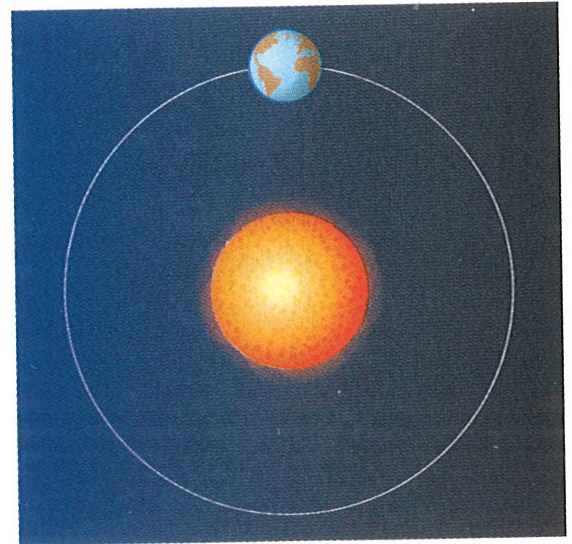
\includegraphics[scale=0.5]{terre}
\end{center}

\begin{questions}
	\question[2] Quelle est la distance parcourue par la Terre autour du Soleil pendant une année ?
	\fillwithdottedlines{3cm}
	
	\question[2] Calculer la vitesse de rotation de la Terre en km/h puis en km/s.
	\fillwithdottedlines{3cm}
\end{questions}


\section{Phrases à compléter (3 points)}

Recopier et compléter les phrases suivantes :

\begin{questions}
	\question[\half] Dans un circuit, plus la résistance augmente, plus l'intensité du courant $....$ .
	\begin{solution}
		Dans un circuit, plus la résistance augmente, plus l'intensité du courant \textbf{diminue}.
	\end{solution}
	
	\question[1] La résistance électrique se mesure à l'aide d'un $....$ et s'exprime en $....$ .
	\begin{solution}
		La résistance électrique se mesure à l'aide d'un \textbf{ohmmètre} et s'exprime en \textbf{ohm} .
	\end{solution}
	
	\question[1\half] La tension aux bornes d'un conducteur ohmique est $....$ à l'intensité du courant qui le traverse : c'est la loi d'Ohm, que l'on traduit par la relation : $....$ = $R$ $\times$  $....$.
	
	\begin{solution}
		La tension aux bornes d'un conducteur ohmique est \textbf{proportionnelle} à l'intensité du courant qui le traverse : c'est la loi d'Ohm, que l'on traduit par la relation : $\mathbf{U}$ = $R$ $\times$  $\mathbf{I}$.
	\end{solution}
\end{questions}

\section{Les lampes à lave (5 points)}

Certaines boutiques vendent des lampes décoratives, appelées <<lampes à lave>>. La chaleur dégagée par l'ampoule située dans le pied de la lampe fait fondre une cire colorée solide. Celle-ci se déplace alors dans une colonne contenant de l'alcool.

\begin{multicols}{2}
	\begin{questions}
		\question[1\half] La cire solide est-elle soluble dans l'alcool ?
		
		\question[1\half] Quel changement d'état subit la cire lorsque la lampe fonctionne ?
		
		\question[2] L'alcool et la cire sont-ils miscibles ?
	\end{questions}

	\begin{center}
		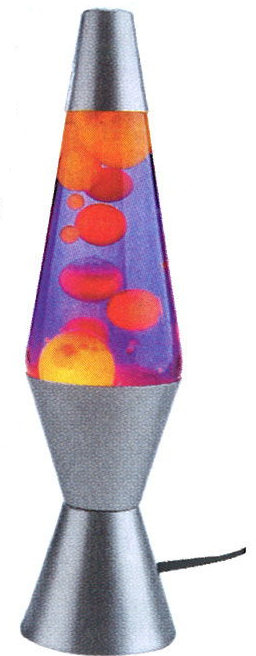
\includegraphics[scale=0.8]{img/lampe}
	\end{center}
\end{multicols}


\section{Cocktail à étages}

Pour épater ses amis, Camille prépare délicatement un cocktail à base de jus d'orange et de sirop de grenadine sans remuer. Arthur regarde le verre et en déduit que le sirop et le jus d'orange ne sont pas miscibles.

\begin{questions}
	\question Explique pourquoi la conclusion d'Arthur est incorrecte ?
	
	\question Comment pourrais-tu lui démontrer son erreur ?
	
	\question Comment peut-on qualifier le mélange de jus d'orange et de sirop après agitation ?
\end{questions}


\section{Lait en poudre (6 points)}

Pour reconstituer du lait de croissance pour bébé, il est indiqué un dosage à respecter impérativement :
\begin{itemize}
	\item <<Une mesurette (\num{4.6} g) de poudre de lait dans 30 mL d'eau. >>	
\end{itemize}

\begin{questions}
	\question[1] Quel est le soluté ?
	
	\question[1] Quel est le solvant ?
	
	\question[2] Combien de mesurettes faut-il dissoudre dans 240 mL d'eau ?
	
	\question[2] Quelle est la masse\footnote{La masse volumique de l'eau est 1 $kg/L$} de la solution obtenue ? 
\end{questions}

\section{Et la température dans tout ça ?}

Le graphique ci-dessous représente la solubilité du  sel (ou chlorure de sodium) dans l'eau en fonction de la température.

\begin{questions}
	\question Complète le graphique en indiquant les grandeurs représentées en abscisse et en ordonnée.
	
	\begin{center}
		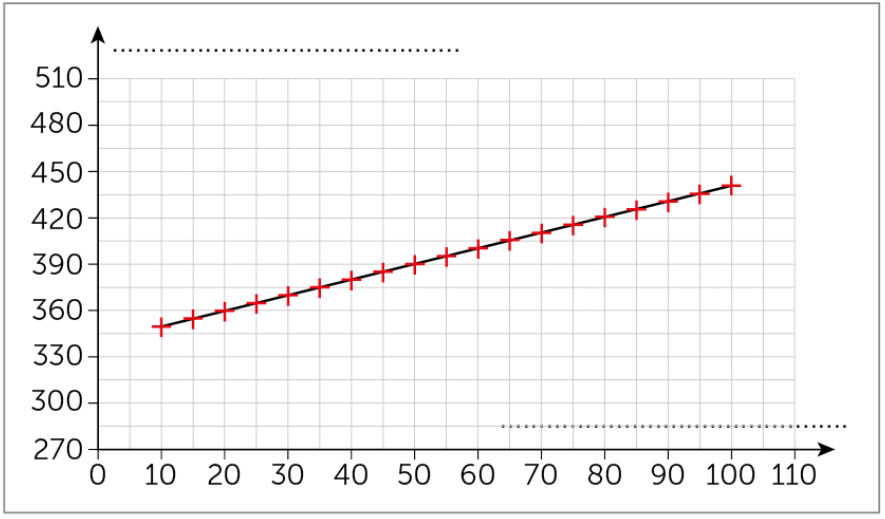
\includegraphics[scale=0.5]{img/courbe}
	\end{center}

	\question \`A $20 °C$, quelle masse de chlorure de sodium peut-on dissoudre au maximum dans 1L de solution ?
	
	\question \`A $90 °C$, quelle masse de chlorure de sodium peut-on dissoudre au maximum dans 1L de solution ?
	
	\question De quoi dépend la solubilité du sel dans l'eau ?
\end{questions}


\ \label{LastPage}

\end{document}